% Modelo de Monografia da Pos Graduacao da PUC - Alterado para cumprir a normalização de 2011
%\documentclass[a4paper,brazil,ruledheader,normaltoc,capchap]{abnt}

% Para impressão frente e verso (normalização 2011)
\documentclass[a4paper,brazil,ruledheader,normaltoc,capchap,twoside,openany]{abnt}

% Não esquecer das alterações no arquivo abnt.cls
% Se estiver usando o Kile no Ubuntu o arquivo fica armazenado em /usr/share/texmf/tex/latex/abntex.
% Comentar a linha 967
% \vspace*{30pt}% - Linha comentada para reduzir o espaçamento entre o topo da página e o título \chapter
% Alterar a linha 1143
% \vspace*{-30pt} % - Parâmetro alterado de 30pt para -30pt para reduzir o espaçamento entre o top da página e o título do apêndice
% Alterar a linha 985
%\vspace*{-30pt}\par % - Parâmetro alterado de 0pt para -30pt para reduzir o espaçamento entre o top da página e o título \chapter*
% Alterar a linha 991
% Parâmetro alterado de 45pt para 30pt para reduzir o espaçamento entre o texto e o título \chapter*

% Não esquecer das alterações no arquivo acronym.sty
% Se estiver usando o Kile no Ubuntu o arquivo fica armazenado em /usr/share/texmf-texlive/tex/latex/acronym
% Alterar a linha 225
%\item[\protect\AC@hypertarget{#1}{\acsfont{\normalfont{#2}}} --] #3% - Inserir separador entre acrônimo/descrição e remover o negrito com o normalfont

% Pacote para definir explicitamente as margens das páginas
\usepackage[a4paper,left=3cm,right=2cm,top=3cm,bottom=2cm]{geometry}

% Pacote para divisão silábica do português
\usepackage[T1]{fontenc}
\usepackage{ae}
\usepackage[utf8x]{inputenc}

%\usepackage{units}
% Utilize da seguinte forma \unit[78,6]{mA}

% Pacote para gerenciar siglas
\usepackage[printonlyused]{acronym}

% Merge em duas células (linhas diferentes)
\usepackage{multirow}

% Pacote para citação e referências seguindo ABNT no sistema (AUTOR, Data)
%\usepackage[alf, bibjustif,abnt-emphasize=bf]{abntcite}
\usepackage[alf, abnt-emphasize=em, abnt-thesis-year=title]{abntcite}
% @article An article from a journal or magazine
% @inproceedings An article in a conference proceedings
% Força que o tipo de ênfase no nome do simpósio seja em caixa alta
\renewcommand{\emph}{\textsc}

% Pacote para múltiplos arquivos .bib
\usepackage{multibib}
%\newcites{pub}{Refer\^encias das publica\c{c}\~oes}

% Pacotes de codificação das fontes para português
\usepackage[brazil]{babel}

% Pacote de adequação do formato ABNT para normas da PUCMinas
\usepackage{abnt-PPGInf-PUCMG}

% Pacotes utilitários
\usepackage[pdftex]{graphicx}
\usepackage{epstopdf}

% Pacote para fixar a figura no local desejado
\usepackage{float}

% Pacote para adicionar simbolos as informações de rodapé
\usepackage[symbol]{footmisc}

\usepackage[all]{xy}
%\usepackage[tight]{subfigure}	% Permite a criação de subfiguras
\usepackage{url,amsmath}	% Permite melhorias na codificação de fórmulas
%\usepackage{amsthm}		% Permite melhorias na escrita de teoremas
\usepackage{amssymb}		% Permite utlização de simbolos matemáticos avançados

\usepackage[portuguese, linesnumbered, ruled, vlined]{algorithm2e}
\usepackage{algorithmic} 	% para algoritmos
\usepackage{listings} 		% para importação de código-fonte

% Alterar o espaçamento da margem no algoritmo
\setlength{\algomargin}{1em}

\usepackage{setspace}

% Pacote para rotação de tabelas/figuras
\usepackage{rotating}

% Pacotes para criação de cronograma/tabela colorida
\usepackage{pstricks}
\usepackage{color}
\usepackage{array}
\usepackage{longtable}
\usepackage{colortbl}
%\definecolor{lightgray}{gray}{0.9}

% Pacote para possibilitar o uso do setboolean para forçar formatos de página diferentes do padrão do documento
\usepackage{ifthen}

% Para inserir captions (nova normalização 2011)
\usepackage[size=normalsize,labelfont=bf,textfont={bf},labelsep=endash]{caption}
\captionsetup[subfloat]{labelfont=bf,textfont={bf}}

% Usado para reduzir espaçamentos entre itens (alíneas, enumerações) com o compactitem
\usepackage{paralist}

% Alterar para sequencial a numeração de figuras e tabelas
\captionsetup{figurewithin=none}
\captionsetup{tablewithin=none}

\setlength{\LTcapwidth}{\textwidth}

% Para o subsubsection aparecer no sumário
\setcounter{tocdepth}{3}
\setcounter{secnumdepth}{3}

% Para inserir referências via links - não funciona para abntex
%\usepackage[colorlinks=true,pdfstartview=FitV,linkcolor=blue,citecolor=blue,urlcolor=blue,hyperindex,pagebackref=true,pdftex,breaklinks]{hyperref}
%\usepackage[pdftex]{hyperref}

% Para criar lista de gráficos
\floatstyle{plaintop}
\newfloat{grafico}{H}{loq}
\restylefloat*{grafico}
\floatname{grafico}{Gráfico}

% Para gerar subfiguras usando o subfloat
\usepackage{subfig}
\newsubfloat[position=bottom,listofformat=subsimple]{grafico}

% define estilo de posicionamento na caixa
\newsavebox{\leftfig}
\newsavebox{\rightfig}

\makeatletter
%\renewcommand{\ALG@name}{Algoritmo}
%\renewcommand{\listalgorithmname}{Lista de Algoritmos}

% Configuração de código-fonte
\lstset{extendedchars=\true, % permite acentos
 inputencoding=utf8x,
 literate={\$}{{\$}}1,
 commentstyle=\it, % deixa os comentários em itálico
 stringstyle=\bf, % não lembro o que faz, mas está funcionando
 belowcaptionskip=5pt, % não lembro o que faz, mas está funcionando
 numbers=left, % coloca a numeração na esquerda
 stepnumber=1, % passos da numeração
 firstnumber=1, % primeira linha
 numberstyle=\tiny, % tamanho da fonte da numeração
 breaklines=true, % permitir quebra de linha
 frame=none, % borda em cima e em baixo
 basicstyle=\small, % estilo básico
 stringstyle=\ttfamily, % não lembro o que faz, mas está funcionando
 showstringspaces=false, % não mostrar os espaços
 mathescape, % não lembro o que faz, mas está funcionando
 tabsize=4 % tamanho da tabulação
}
\renewcommand{\thefootnote}{\arabic{footnote}}
\renewcommand{\lstlistingname}{Código}
\renewcommand{\lstlistlistingname}{Lista de Códigos}
\citeoption{abnt-etal-cite=1, abnt-and-type=e}

\lstdefinelanguage{Scala}{
  morekeywords={%
          abstract,case,catch,class,def,do,else,extends,%
          false,final,finally,for,forSome,if,implicit,import,lazy,%
          match,new,null,object,override,package,private,protected,%
          return,sealed,super,this,throw,trait,true,try,type,%
          val,var,while,with,yield},
  otherkeywords={=>,<-,<\%,<:,>:,\#,@},
  sensitive=true,
  morecomment=[l]{//},
  morecomment=[n]{/*}{*/},
  morestring=[b]",
  morestring=[b]',
  morestring=[b]"""
}[keywords,comments,strings]

\lstdefinelanguage{Clojure}%
{morekeywords={*,*1,*2,*3,*agent*,*allow-unresolved-vars*,*assert*,*clojure-version*,*command-line-args*,%
*compile-files*,*compile-path*,*e,*err*,*file*,*flush-on-newline*,*in*,*macro-meta*,%
*math-context*,*ns*,*out*,*print-dup*,*print-length*,*print-level*,*print-meta*,*print-readably*,%
*read-eval*,*source-path*,*use-context-classloader*,*warn-on-reflection*,+,-,->,->>,..,/,:else,%
<,<=,=,==,>,>=,@,accessor,aclone,add-classpath,add-watch,agent,agent-errors,aget,alength,alias,%
all-ns,alter,alter-meta!,alter-var-root,amap,ancestors,and,apply,areduce,array-map,aset,%
aset-boolean,aset-byte,aset-char,aset-double,aset-float,aset-int,aset-long,aset-short,assert,%
assoc,assoc!,assoc-in,associative?,atom,await,await-for,await1,bases,bean,bigdec,bigint,binding,%
bit-and,bit-and-not,bit-clear,bit-flip,bit-not,bit-or,bit-set,bit-shift-left,bit-shift-right,%
bit-test,bit-xor,boolean,boolean-array,booleans,bound-fn,bound-fn*,butlast,byte,byte-array,%
bytes,cast,char,char-array,char-escape-string,char-name-string,char?,chars,chunk,chunk-append,%
chunk-buffer,chunk-cons,chunk-first,chunk-next,chunk-rest,chunked-seq?,class,class?,%
clear-agent-errors,clojure-version,coll?,comment,commute,comp,comparator,compare,compare-and-set!,%
compile,complement,concat,cond,condp,conj,conj!,cons,constantly,construct-proxy,contains?,count,%
counted?,create-ns,create-struct,cycle,dec,decimal?,declare,def,definline,defmacro,defmethod,%
defmulti,defn,defn-,defonce,defprotocol,defstruct,deftype,delay,delay?,deliver,deref,derive,%
descendants,destructure,disj,disj!,dissoc,dissoc!,distinct,distinct?,do,do-template,doall,doc,%
dorun,doseq,dosync,dotimes,doto,double,double-array,doubles,drop,drop-last,drop-while,empty,empty?,%
ensure,enumeration-seq,eval,even?,every?,false,false?,ffirst,file-seq,filter,finally,find,find-doc,%
find-ns,find-var,first,float,float-array,float?,floats,flush,fn,fn?,fnext,for,force,format,future,%
future-call,future-cancel,future-cancelled?,future-done?,future?,gen-class,gen-interface,gensym,%
get,get-in,get-method,get-proxy-class,get-thread-bindings,get-validator,hash,hash-map,hash-set,%
identical?,identity,if,if-let,if-not,ifn?,import,in-ns,inc,init-proxy,instance?,int,int-array,%
integer?,interleave,intern,interpose,into,into-array,ints,io!,isa?,iterate,iterator-seq,juxt,%
key,keys,keyword,keyword?,last,lazy-cat,lazy-seq,let,letfn,line-seq,list,list*,list?,load,load-file,%
load-reader,load-string,loaded-libs,locking,long,long-array,longs,loop,macroexpand,macroexpand-1,%
make-array,make-hierarchy,map,map?,mapcat,max,max-key,memfn,memoize,merge,merge-with,meta,%
method-sig,methods,min,min-key,mod,monitor-enter,monitor-exit,name,namespace,neg?,new,newline,%
next,nfirst,nil,nil?,nnext,not,not-any?,not-empty,not-every?,not=,ns,ns-aliases,ns-imports,%
ns-interns,ns-map,ns-name,ns-publics,ns-refers,ns-resolve,ns-unalias,ns-unmap,nth,nthnext,num,%
number?,odd?,or,parents,partial,partition,pcalls,peek,persistent!,pmap,pop,pop!,pop-thread-bindings,%
pos?,pr,pr-str,prefer-method,prefers,primitives-classnames,print,print-ctor,print-doc,print-dup,%
print-method,print-namespace-doc,print-simple,print-special-doc,print-str,printf,println,println-str,%
prn,prn-str,promise,proxy,proxy-call-with-super,proxy-mappings,proxy-name,proxy-super,%
push-thread-bindings,pvalues,quot,rand,rand-int,range,ratio?,rational?,rationalize,re-find,%
re-groups,re-matcher,re-matches,re-pattern,re-seq,read,read-line,read-string,recur,reduce,ref,%
ref-history-count,ref-max-history,ref-min-history,ref-set,refer,refer-clojure,reify,%
release-pending-sends,rem,remove,remove-method,remove-ns,remove-watch,repeat,repeatedly,%
replace,replicate,require,reset!,reset-meta!,resolve,rest,resultset-seq,reverse,reversible?,%
rseq,rsubseq,second,select-keys,send,send-off,seq,seq?,seque,sequence,sequential?,set,set!,%
set-validator!,set?,short,short-array,shorts,shutdown-agents,slurp,some,sort,sort-by,sorted-map,%
sorted-map-by,sorted-set,sorted-set-by,sorted?,special-form-anchor,special-symbol?,split-at,%
split-with,str,stream?,string?,struct,struct-map,subs,subseq,subvec,supers,swap!,symbol,symbol?,%
sync,syntax-symbol-anchor,take,take-last,take-nth,take-while,test,the-ns,throw,time,to-array,%
to-array-2d,trampoline,transient,tree-seq,true,true?,try,type,unchecked-add,unchecked-dec,%
unchecked-divide,unchecked-inc,unchecked-multiply,unchecked-negate,unchecked-remainder,%
unchecked-subtract,underive,unquote,unquote-splicing,update-in,update-proxy,use,val,vals,%
var,var-get,var-set,var?,vary-meta,vec,vector,vector?,when,when-first,when-let,when-not,%
while,with-bindings,with-bindings*,with-in-str,with-loading-context,with-local-vars,%
with-meta,with-open,with-out-str,with-precision,xml-seq,zero?,zipmap
},%
   sensitive,% ???
   alsodigit=-,%
   morecomment=[l];,%
   morestring=[b]"%
  }[keywords,comments,strings]%

\pdfinfo{%
  /Title    (Vantagens de uso da programação funcional dentro da plataforma Java)
  /Author   (Rodrigo Lazoti da Silva)
  /Creator  (Rodrigo Lazoti da Silva)
  /Producer (Kile - an Integrated LaTeX Environment - Version 2.0.85)
  /Subject  (Monografia de Pós Graduação)
  /Keywords ()
}

%%%%%%%%%%%%%%%%%%%%%%%%%%%% PRÉ-TEXTUAIS %%%%%%%%%%%%%%%%%%%%%%%%%%
\begin{document}

% Para forçar que elementos pré-textuais (da capa até o sumário) sejam impressos no anverso da folha
\setboolean{@twoside}{false}

\autor{Rodrigo Lazoti da Silva}

% Coloque o título em caixa alta. É o padrão da PUC.
% Vá no arquivo abnt-PPGInf-PUCMG.sty e procure por esse título (linha 575). Altere para o seu título em caixa alta. Isso será utilizado na folha de aprovação.
\titulo{VANTAGENS DE USO DA PROGRAMAÇÃO FUNCIONAL DENTRO DA PLATAFORMA JAVA}

\orientador[Orientador:]{Prof. Carlos Barreto Ribas}

% Se não tiver, co-orientador, comente a próxima linha.
%\coorientador[Co-orientador:]{Professor}

% Texto


\comentario{Monografia apresentada ao Curso de Pós- Graduação em Engenharia de Software da Pontifícia Universidade Católica de Minas Gerais, como requisito parcial para obtenção do título de Especialista em Engenharia de Software.}

% Instituição
\instituicao{Pós Graduação em Engenharia de Software \par Pontifícia Universidade Católica de Minas Gerais}

% Local
\local{Belo Horizonte}

% Data
\data{2013}

% Gera a capa
\capa

% Para forçar que a ficha catalográfica seja impressa no verso da folha de aprovação
% \setboolean{@twoside}{true}

% Gera a folha de rosto
\folhaderosto

% Ficha catalográfica
%\include{pre-texto/ficha-catalografica}

% Para forçar que elementos pré-textuais (da capa até o sumário) sejam impressos no anverso da folha
\setboolean{@twoside}{false}

% Folha de aprovação
% Termo de Aprovação

% Texto da aprovação
\textoaprovacao{Monografia apresentada ao Curso de Pós- Graduação em Engenharia de Software da Pontifícia Universidade Católica de Minas Gerais, como requisito parcial para obtenção do título de Especialista em Engenharia de Software.}

% Primeira assinatura
\primeiroassina{Prof. Carlos Barreto Ribas (Orientador) -- PUC Minas}

% Segunda assinatura
\segundoassina{Prof. Humberto Torres Marques Neto -- PUC Minas}

% Terceira assinatura
% \terceiroassina{Prof. Dr. Membro externo -- Instituição}

% Quarta assinatura
%\quartoassina{}

% Data da defesa
\localdia{Belo Horizonte, 10 de dezembro de 2013}

% Gera o termo de aprovação
\termodeaprovacao


% Dedicatória
% Dedicatória
\newpage

% Espaçamento do topo da página até o texto da dedicatória
\vspace*{20cm}

\hspace{8cm}
\begin{minipage}{.45\textwidth}
\textit{À minha esposa Andressa pelo seu apoio incondicional, ao meu filho Rafael pela sua compreensão e paciência e à minha mãe por todo o seu apoio.}
\end{minipage}


% Agradecimentos
% Agradecimentos
%\chapter*{Agradecimentos}
\begin{center}
	\normalsize
	\textbf{AGRADECIMENTOS}
\end{center}

  À todos que de alguma forma contribuíram para esta construção deste trabalho.

  Aos grandes colegas e amigos do curso de Pós-Graduação em Engenharia de Software da Pontifícia Universidade Católica De Minas Gerais pela excelente amizade consolidada neste período.

  Ao corpo docente do curso de Pós-Graduação em Engenharia de Software da Pontifícia Universidade Católica De Minas Gerais pelo apoio e pelas sugestões que muito me auxiliaram na elaboração deste trabalho.


% Epígrafe
% Epígrafe
\newpage

% Espaçamento entre topo da página e texto da epígrafe
\vspace*{10cm}
% Espaçamento na esquerda
\hspace{4cm}\begin{minipage}{.51\textwidth}

% Texto da epígrafe
\textit{Seu tempo é limitado, então não o desperdice vivendo a vida de outra pessoa. Não fique preso pelo dogma - que é viver pelos resultados do que outras pessoas pensam. Não deixe o ruído da opinião dos outros afogar a sua voz interior. E o mais importante, tenha a coragem de seguir seu coração e sua intuição. Eles de alguma forma já sabem o que você realmente quer se tornar. Tudo o mais é secundário.\cite{Jobs}}

%Nome do autor
% \begin{flushright}\itshape Steve Jobs \upshape\end{flushright}

\end{minipage}


% Resumo
% Resumo
\begin{resumo}
% Diminuir espaçamento entre título e texto
\vspace{-1cm}

% Texto do resumo: sem paragrafo, justificado, com espaçamento 1,5 cm
\onehalfspacing

\noindent
  %objetivo e metodo
  Esta monografia realizou um experimento sobre o uso das linguagens de programação Clojure e Scala na máquina virtual Java. O objetivo foi analisar através de métricas o uso dessas linguagens que utilizam o paradigma da programação funcional na escrita de determinados tipos de algoritmos e que foram comparados com algoritmos escritos com a linguagem padrão da máquina virtual Java que é a linguagem de programação Java, e que faz uso do paradigma de programação orientado a objetos. A avaliação comparativa utilizou como métricas para comparação a quantidade de linhas de cada algoritmo, e o tempo em milissegundos de execução gasto por cada algoritmo.

  %resultado e conclusoes
  Após análise dos dados coletados pelo experimento proposto nesse trabalho, os resultados mostram que utilizando linguagens de programação funcional como Clojure ou Scala na máquina virtual Java, consegue-se obter um melhor desempenho em algoritmos que precisam fazer cálculos ou iterar sobre listas de objetos e também de escrever menos código para se obter os resultados desejados.

% Espaçamento para as palavras-chave
\vspace*{.75cm}

% Palavras-chave: sem parágrafo, alinhado à esquerda
\noindent Palavras-chave: Programação funcional, Programação Orientada a Objetos, Java, Scala, Clojure, máquina virtual Java.\\
% Segunda linha de palavras-chave, com espaçamento.
%\indent\hspace{2cm}Palavra.

\end{resumo}


% Abstract
% Abstract
\begin{abstract}
% Diminuir espaçamento entre título e texto
\vspace{-1cm}
% Texto do resumo, em inglês: sem paragrafo, justificado, com espaçamento 1,5 cm
\onehalfspacing
\noindent
  This monograph conducted an experiment on the use of programming languages ​​Clojure and Scala in the Java virtual machine. The objective was to analyze metrics through the use of these languages ​​using the paradigm of functional programming in writing certain types of algorithms and that were compared to the algorithms written in the standard language of the Java virtual machine which is the Java programming language that it makes use of the paradigm of object-oriented programming. The benchmarking used as metrics to compare the number of lines of each algorithm and the execution time in milliseconds spent by each algorithm.

  After analyzing the data collected by the experiment proposed in this work, the results show that using functional programming languages ​​like Clojure or Scala in the Java virtual machine achieves better performance in algorithms that need doing calculations or iterate over lists of objects, and also to write less code to achieve the desired results.

% Espaçamento para as palavras-chave
\vspace*{.75cm}

% Palavras-chave: sem parágrafo, alinhado à esquerda
\noindent Keywords: Functional Programming, Object Oriented Programming, Java, Scala, Clojure, Java Virtual Machine. \\
% Segunda linha de palavras-chave, com espaçamento.
%\indent\hspace{1.4cm} Keyword.

\end{abstract}


\makeatletter
\renewcommand\numberline[1]{
	\leftskip 0em
	\rightskip 1.6em
	\parfillskip -\rightskip
	\parindent 0em
	\@tempdima 2.0em
	\vspace{0em} \advance\leftskip \@tempdima \null\nobreak\hskip -\leftskip
	FIGURA \normalfont #1 -- }
\makeatother

% Lista de figuras
% \listoffigures

\makeatletter
\renewcommand\numberline[1]{
	\leftskip 0em
	\rightskip 1.6em
	\parfillskip -\rightskip
	\parindent 0em
	\@tempdima 2.0em
	\vspace{0em} \advance\leftskip \@tempdima \null\nobreak\hskip -\leftskip
	TABELA \normalfont #1 -- }
\makeatother

% Lista de tabelas
\listoftables

% \makeatletter
% \renewcommand\numberline[1]{
% 	\leftskip 0em
% 	\rightskip 1.6em
% 	\parfillskip -\rightskip
% 	\parindent 0em
% 	\@tempdima 2.0em
% 	\vspace{0.5em} \advance\leftskip \@tempdima \null\nobreak\hskip -\leftskip
% 	GRÁFICO \normalfont #1 -- }
% \makeatother

% Lista de graficos
\listof{grafico}{Lista de Gráficos}

% Lista de siglas
% Lista de Abreviaturas e Siglas
%\chapter*{Lista de Abreviaturas e Siglas}
\chapter*{Lista de Abreviaturas e Siglas}

% Mantenha sempre em ordem alfabética.

\begin{acronym}
\acro{EPFL}   {\textit{École Polytechnique Fédérale de Lausanne}}
\acro{FP}     {\textit{Functional Programming - Programação Funcional}}
\acro{JDK}    {\textit{Java Developer Kit}}
\acro{JVM}    {\textit{Java Virtual Machine - Máquina Virtual Java}}
\acro{Lisp}   {\textit{List Processing - Processador de listas}}
\acro{LoC}    {\textit{Lines of Code - Linhas de Código}}
\acro{OOP}    {\textit{Object Oriented Programming - Programação Orientada a Objetos}}
\acro{opcode} {\textit{Operation Code - Código de instrução}}
\acro{TCO}    {\textit{tail call optimization}}
\acro{TI}     {\textit{Tecnologia da Informação}}

\end{acronym}


\makeatletter
\renewcommand\numberline[1]{#1\hspace{0.8em}}
\makeatother

% Altera para espaçamento simples a partir daqui
\singlespacing

% Sumário
\tableofcontents

% Altera para espaçamento 1,5 a partir daqui
\onehalfspacing

%%%%%%%%%%%%%%%%%%%%%%%%%%%%% TEXTUAIS %%%%%%%%%%%%%%%%%%%%%%%%%%%
% Para forçar que elementos textuais e pós-textuais sejam impressos no anverso e verso das folhas
\setboolean{@twoside}{true}
% Altere o número da página para o correto. Conte todas as páginas frente e verso, menos a capa, nclusive a ficha catalográfica até a página do primeiro capítulo.
\setcounter{page}{25}

% Capítulos
% Para forçar que o capítulo de introdução comece no anverso
\setboolean{@openright}{true}
\chapter{Introdução}

\vspace{-1.9cm}

Desde o surgimento da máquina virtual Java, a linguagem de programação Java vem sendo utilizada para desenvolver sistemas para as mais diversas finalidades utilizando o paradigma de programação orientada a objetos, porém nos últimos anos surgiram outras linguagens de programação que conseguem gerar bytecode Java e que por sua vez podem ser executadas dentro da máquina virtual Java. Algumas dessas linguagens tem como base o paradigma da programação funcional, sendo que as que mais se destacam são as linguagens Clojure e Scala.

Um ponto interessante a se considerar entre as linguagens de programação Clojure e Scala e a própria linguagem de programação Java é que mesmo utilizando paradigmas de programação distintos ainda existe interoperabilidade entre elas e que com isso é possível compartilhar algoritmos e invocar códigos escritos entre estas linguagens de programação.

\section{Justificativa}

  Embora a primeira vista pareça interessante utilizar em um mesmo projeto linguagens funcionais como Scala ou Clojure em conjunto com a linguagem Java, faz-se necessário um estudo para avaliar e descobrir em quais circunstâncias algoritmos escritos através da programação funcional possuem vantagem sobre algoritmos que produzem os mesmos resultados, mas que foram escritos através da programação orientada a objetos.

  A principal justificativa para a realização desta pesquisa é demonstrar o uso da programação funcional dentro da máquina virtual Java através das linguagens Clojure e Scala, e as vantagens que pode-se obter ao optar pelo uso dessas linguagens.

\section{Objetivos}

  \subsection{Objetivo Geral}

    O principal objetivo desse trabalho é introduzir o paradigma da programação funcional, sua essência e a sua utilização dentro da plataforma Java, assim como demonstrar a viabilidade de uso do paradigma funcional na escrita de algoritmos e também expor sua simplicidade, melhor legibilidade e desempenho para determinadas tarefas.

  \subsection{Objetivos Específicos}

    \begin{compactitem}
      \item Contextualizar os princípios do paradigma da programação funcional e da programação orientada a objetos.
      \item Introduzir o uso da programação funcional dentro da plataforma Java por meio das linguagens Clojure e Scala;
      \item Introduzir o uso da interoperabilidade entre linguagens de programação dentro da plataforma Java;
      \item Como aplicar testes comparativos de desempenho e de como avaliar a legibilidade em algoritmos escritos em Clojure, Java e Scala;
    \end{compactitem}

\section{Problema}

  Observa-se a necessidade do mercado pelo rápido desenvolvimento de aplicações e em conjunto uma grande dificuldade dos desenvolvedores para acompanhar essa velocidade na implementação de algoritmos que proporcionem ao mesmo tempo simplicidade na codificação e ganho de desempenho. Algumas linguagens de programação não oferecem uma flexibilidade na codificação de algoritmos, gerando muito mais código e consequentemente dificultando o seu entendimento e a sua facilidade de manutenção.

\section{Metodologia}

  A modalidade de trabalho proposta para esta pesquisa é utilizar o formato de experimento, para assim conseguir realizar testes com a utilização de dois paradigmas de programação distintos e de mudanças em como algoritmos são escritos mesclando o uso de diferentes paradigmas de programação em uma única plataforma.

  O método de pesquisa aplicado será uma avaliação comparativa entre dois paradigmas de programação.

  O método de abordagem aplicado nesta pesquisa será uma abordagem indutiva e qualitativa, para que a pesquisa explore e apresente uma análise com base nos dados obtidos pela avaliação comparativa.

\section{Organização do Documento}

  O primeiro capítulo contém uma breve introdução sobre esta monografia, a descrição das motivações, interesses e objetivos utilizados para compor esta monografia.

  No segundo capítulo apresenta-se o que são paradigmas de programação e descreve-se também o paradigma de programação funcional e o paradigma de programação orientada a objetos.

  O terceiro capítulo apresenta a máquina virtual Java, o bytecode Java e a interoperabilidade entre linguagens de programação na plataforma Java.

  No quarto capítulo apresenta-se as linguagens de programação Clojure, Scala e Java.

  O quinto capítulo apresenta os programas utilizados nos experimentos.

  O sexto capítulo apresenta a execução dos programas apresentados no capítulo anterior, assim como os resultados obtidos por eles.

  O sétimo capítulo apresenta a conclusão obtida através do experimento realizado nesse trabalho.

% Os demais capítulos não precisam começar no anverso
\setboolean{@openright}{false}
\chapter{Paradigmas de Programação}

\vspace{-1.9cm}

``Paradigma é um termo com origem no grego \"paradeigma\" que significa modelo, padrão. No sentido lato corresponde a algo que vai servir de modelo ou exemplo a ser seguido em determinada situação. São as normas orientadoras de um grupo que estabelecem limites e que determinam como um indivíduo deve agir dentro desses limites.'' \cite{Significados:2013}.

Paradigma de programação pode ser definido como um uma idéia que o desenvolvedor possui ao estruturar e escrever um programa. Metodologias diferentes são propostas através de diferentes linguagens de programação, sendo que estas apresentam diferentes paradigmas. Um paradigma de programação está relacionado à maneira de pensar do desenvolvedor e na forma em que ele escreve uma solução para os problemas. É através do paradigma que permite-se ou proíbe-se o uso de determinadas técnicas de programação.

Paradigmas de programação são classificados com base em seus conceitos que podem ser: estruturado, funcional, imperativo, lógico e orientado a objetos. Cada paradigma define uma forma particular de tratar problemas e de definir possíveis soluções. Fora isso, uma linguagem de programação pode fazer uso de mais de um paradigma para melhorar as análises e soluções.

\section{Programação Funcional}

  Segundo Fogus ``Programação funcional é o uso de funções que transformam valores em unidades de abstração, subsequentemente usadas para construir sistemas de software.''(FOGUS, 2013, tradução nossa).\nocite{FuncJS:2013}\footnote{Functional programming is the use of functions that transform values into units of abstraction, subsequently used to build software systems.}

  O Paradigma de programação funcional basicamente cria algoritmos escritos em linguagem definida por expressões, declarações e funções, considerando a computação como uma avaliação de funções matemáticas. Com o uso da \ac{FP} existe também a possibilidade de escrever algoritmos onde podemos determinar o que se pretende criar e não como será criado. O paradigma funcional não utiliza o conceito de atribuição pelo fato de que os programas são formados por definições de funções. Uma de suas características determinantes é a aplicação de funções à dados imutáveis e sem estados.

  Existem inúmeras características que cada linguagem funcional utiliza, mas geralmente as linguagens de programação funcionais tem as seguintes características:

  \begin{compactitem}
    \item Funções de ordem superior;
    \item Transparência referencial;
    \item Recursão;
    \item Imutabilidade;
  \end{compactitem}

  Na área da matemática e da ciência da computação, funções de ordem superior são funções que podem receber funções como argumentos, assim como produzir funções como resultado de sua computação. Por ser um modelo simples, o cálculo lambda permite demonstrar alguns conceitos importantes de linguagens de programação, como por exemplo ligação, escopo, ordem de avaliação, computabilidade, sistemas de tipos e etc.\cite{fpjava}.

  Na matemática, funções nunca possuem efeitos colaterais. Por exemplo, não importa o que aconteça internamente em um método chamado $cos(x)$ que calcule o co-seno de $x$, o resultado será sempre o mesmo para um dado valor de $x$, sem nenhuma mudança no estado externo do programa que invocou este método. Por exemplo, dado a função $y = f x$ e a função $g = h y y$, é possível substituir a definição de $g$ pela função $g = h (f x) (f x)$ e obter o mesmo resultado. Estar apto a substituir a chamada de uma função por um conjunto de parâmetros com o valor esperado é chamada de transparência referencial e torna possível conduzir o raciocínio equacional no código.\cite{Haskell:2013}.

  Recursão é um recurso amplamente utilizado na programação funcional como a principal forma de iteração. Linguagens de programação funcionais frequentemente irão oferecer otimizações para garantir que a execuções de recursões grandes não consumam muita memória sem necessidade.\cite{Haskell:2013}.

  Programas funcionais puros tipicamente operam através de dados imutáveis, dados que não possuem mudança de valor. Ao invés de alterar valores existentes dos dados, são criadas cópias alteradas e os valores originais são mantidos. Desde que a estrutura desses dados não possam ser modificadas, eles podem frequentemente ser compartilhados entre cópias novas e velhas armazenadas em memória.

  \subsection{Cálculo Lambda}
    O calculo lambda também conhecido pelo símbolo $\lambda$, foi inventado por Alonzo Chruch em 1930 e publicado em 1941 em resposta ao problema de decisão de David Hilbert (Hilbert's Entscheidungsproblem) proposto no ano de 1928. O problema de decisão inspirou outro modelo computacional conhecido como máquina de Turing.\cite{WhatsLC:2013}

    O calculo lambda é um dos pilares da ciência da computação e pode ser considerado a primeira linguagem de programação funcional, embora nunca tenha sido projetada para ser realmente executada em um computador. Ele talvez seja o mais famoso, por servir como base para a linguagem de programação LISP, inventada por John McCarthy em 1958.\cite{WhatsLC:2013}

    O cálculo lambda é um modelo matemático, e pode ser pensado como uma linguagem de programação pura, baseada na definição e aplicação de funções, e o seu método de iteração é através da recursão. Esse modelo permite a representação de qualquer algoritmo, e é pura no sentido de que as funções recebem e retornam dados, que podem ser inclusive funções, e não podem ser alterados pela função.\nocite{FormalLC:2013}

    Funções em cálculo lambda são muito diferentes de funções em linguagens de programação imperativas como Java e C. Em uma linguagem de programação imperativa a avaliação de uma função pode ter efeitos colaterais, afetando avaliações futuras de uma função para outras funções. No cálculo lambda uma função não pode retornar um resultado baseado em seus parâmetros, as invés disso seus parâmetros são reduzidos para chegar em um resultado que matematicamente é equivalente a questão.\cite{IntroLambda:1989}.

    O conceito central em cálculo lambda são as expressões ou termos, sendo que existem três tipos de expressões:

    \begin{compactitem}
      \item Variável: x;
      \item Abstração ou Função: $\lambda$x.e;
      \item Aplicação: x y;
    \end{compactitem}

    Variáveis são expressas por meio de identificadores alfanuméricos, com por exemplo a letra $x$. Abstrações representam a função que retorna o valor $e$ quando recebe o parâmetro formal $x$, sendo que o $.$ na expressão separa o argumento da função de seu corpo. Aplicações representam a aplicação da expressão $x$ para $y$.

\section{Programação Orientada a Objetos}

  Paradigma de orientação a objetos é um conceito que foi criado devido a necessidade de ultrapassar os problemas que foram encontrados com o uso de técnicas como a programação estruturada. Enquanto a programação estruturada tem colocado ênfase na lógica e ações, a programação orientada a objetos tomou uma direção completamente diferente colocando ênfase em objetos e informações. Com a programação orientada a objetos, um problema vai ser dividido em várias unidades que são chamados de objetos.

  Existem vantagens ao utilizar a programação orientada a objetos como a manutenção simplificada, uma análise avançada de programas complexos e reutilização de código. Existe uma série de linguagens de programação que usam \ac{OOP}, como o Java, C++ e Smalltalk. Um conceito importante na \ac{OOP} é a modelagem de dados, pois antes de construir um sistema orientado a objetos, é necessário encontrar os objetos dentro do sistema e determinar as relações entre eles.

  Uma classe é uma unidade que armazena dados e funções que irão realizar operações sobre os dados. Um objeto é uma instância de classe e ele pode receber e enviar mensagens para outros objetos. Os objetos que existem dentro de programas são muitas vezes baseados em objetos do mundo real, e que irão se comportar da mesma maneira.

  Existem duas coisas que são encontradas em todos os objetos que existem no mundo real, essas duas coisas são comportamentos e estados. Enquanto comportamentos e estados são encontrados em objetos do mundo real, eles também podem ser codificados para objetos no programa.

  As principais características das linguagens de programação orientadas a objetos são:

  \begin{compactitem}
    \item Herança;
    \item Encapsulamento;
    \item Polimorfismo;
  \end{compactitem}

  Herança é um aspecto da \ac{OOP} que permite que subclasses possam herdar os traços e as características de sua superclasse. A subclasse herdará todos os membros, exceto aqueles que foram definidos como sendo privado. Uma subclasse pode usar o comportamento dos membros que herdou da superclasse e que também pode adicionar novos membros e comportamentos. Existem duas grandes vantagens no uso de herança que são a implementação de dados abstratos e reutilização de comportamentos.

  Encapsulamento é responsável por proteger os dados dentro de uma classe de objetos externos. Ele só irá revelar a informação funcional. No entanto, a implementação será ocultada. O encapsulamento é um conceito que promove a modularidade e é também crucial para esconder informações que não precisam ser expostas para outros objetos.

  Polimorfismo é a capacidade de diferentes objetos para responder à mesma mensagem de diferentes maneiras. Ele permite que um único nome ou o operador a ser associada com diferentes operações, dependendo do tipo de dados que tenha passado, e dá a possibilidade de redefinição de um método dentro de uma classe de derivados.
  \cite{esPratica:2010}

\chapter{Plataforma Java}

\vspace{-1.9cm}

  \section{História do Java}

  Com o Java, a Sun Microsystems criou a primeira linguagem de programação que não estava vinculada a nenhum sistema operacional específico ou microprocessador. As aplicações escritas em Java podiam ser executadas em qualquer lugar, eliminando um dos maiores problemas para os usuários de computador, a incompatibilidade entre sistemas operacionais e versões de sistemas operacionais.

  O Java foi desenvolvido a partir de um desejo de construir software para produtos eletrônicos de consumo como aparelhos eletrônicos e eletrodomésticos. Tudo começou em 1991, quando uma equipe de pesquisadores da Sun desenvolveu alguns conceitos dando uma nova direção para alta tecnologia, os consumidores que necessitavam de computadores estavam por toda a parte e foram a força motriz por trás de muitos dos produtos voltados para a casa como o videocassete, o forno de micro-ondas e o sistema de som. No entanto, cada produto necessitava da sua própria interface. Em outras palavras, para controlar três dispositivos, os consumidores tiveram que ter três controles remotos e compreender o manuseio para os três dispositivos. Além do fato de que a Sun estava ficando para trás de seus concorrentes, este foi um forte motivador para a Sun lançar um novo projeto, que mais tarde se tornaria o Java.\cite{JavaTimeline:2013}.

  Uma equipe chamada Green Team foi formada para trabalhar na criação de um dispositivo simples que controlava uma variedade de produtos eletrônicos de uso para o dia-a-dia. A equipe foi composta por dois programadores, Patrick Naughton e James Gosling, e o engenheiro Mike Sheridan. Gosling percebeu que o que eles precisavam era de uma nova linguagem de programação.\cite{JavaHistory:2013}.

  Até o momento, as linguagens de programação existentes como o C++ tinha sua ênfase na velocidade, e não na confiabilidade. No setor de eletroeletrônicos, a confiabilidade é mais importante que a velocidade. Com este propósito Gosling e Naughton conseguiram realizar o trabalho em conjunto e criar uma nova linguagem que eles chamaram de Oak e isso aconteceu em agosto de 1991. Um ano depois, o Green Team desenvolveu um dispositivo portátil, sem teclado, sem botões e com uma tela minúscula. Bastava um toque para ativá-lo e controlar a ação na tela com a ponta do dedo, e com esse dispositivo tornou-se possível programar o gravador de videocassete apenas movendo o dedo ao longo da tela. Ainda assim, esta tecnologia não emplacou devido a vários motivos como a fabricação dos chips que eram muito caros.\cite{CoreJava:2010}.

  O nome Oak teve de ser alterado devido ao fato de que era muito próximo ao de uma linguagem de programação já existente, consequentemente Oak foi rebatizado como Java. Em 1994, a maioria das pessoas utilizam o Mosaic, um navegador Web não-comercial e em meados de 1994 os desenvolvedores da Sun viram uma oportunidade para a linguagem Java com o surgimento da World Wide Web. Sua idéia era liberar o Java de graça na Internet liberando também o seu próprio navegador para uso não comercial, para que assim eles se tornassem um padrão.\cite{CoreJava:2010}.

\section{Máquina Virtual Java}

  A máquina virtual Java, conhecida também pela sigla \ac{JVM} que é um acrônimo para Java Virtual Machine, é o principal componente da plataforma Java. Ela é a tecnologia responsável por tornar programas escritos em Java independentes de sistemas operacionais e de hardware. A \ac{JVM} é chamada de "virtual", pois fornece uma interface que não depende de sistema operacional subjacente ou da arquitetura de hardware da máquina. Esta independência de hardware e de sistema operacional é a base do termo "Write Once, Run Anywhere" que traduzido significa "escreve uma vez, execute em qualquer lugar"\cite{jvm:2013}. Existem versões da \ac{JVM} para diversas arquiteturas e sistemas operacionais.

  A maioria das linguagens de programação compilam o código fonte diretamente para código de máquina, que é projetado para ser executado em uma arquitetura de microprocessador específico ou sistema operacional, como o Windows ou Unix. No caso da \ac{JVM}, ela permite que o bytecode Java possa ser executado como ações ou chamadas de sistema operacional em qualquer processador, independentemente do sistema operacional. Portanto, a \ac{JVM} não tem conhecimento sobre a linguagem Java, porque ela entende somente o bytecode. Desta forma, qualquer linguagem que possar ser compilada e ser capaz gerar bytecode Java poderá ser executada na \ac{JVM}.

  Algumas das características mais importantes da \ac{JVM} são:

  \begin{compactitem}
    \item Baseia-se numa pilha de avaliação, o qual pode ser manipulada pelos bytecodes Java. Os argumentos do método são enviados para a pilha antes da invocação de um método, e quando completado o valor de retorno está localizado na pilha.
    \item É fortemente tipada.
    \item Manipulação de ponteiro não é permitido.
    \item Possui coleta automática de lixo, onde os objetos não referenciados são automaticamente liberados da memória.
  \end{compactitem}

  \section{Bytecode Java}

  Arquivos $.class$ são o resultado da compilação de programas escritos com a linguagem Java. Os arquivos $.class$ contém bytecode Java, sendo que bytecode Java são instruções que a máquina virtual Java consegue executar, cada instrução ou bytecode a ser executado é um código de operação (\ac{opcode}) com o tamanho de um byte, seguido por zero ou mais operandos fornecendo argumentos ou dados que são usados na operação. Atualmente existem 256 opcodes possíveis, embora nem todos estejam sendo utilizados e mais 51 opcodes estão reservados para uso futuro.\cite{jvm:2013}. Muitas instruções não tem operandos e consiste apenas de um único \ac{opcode}.

  Segundo \citeonline{jvm:2013}, essas instruções são agrupadas da seguinte forma:

  \begin{compactitem}
    \item Operações para checagem de tipos;
    \item Operações de carga e armazenamento;
    \item Operações aritméticas;
    \item Operações para conversão de tipos;
    \item Operações para criação e manipulação de objetos;
    \item Operações para gerenciamento de pilha;
    \item Operações para controle de fluxo;
    \item Operações para invocação de método;
    \item Operações lançamento de exceções;
    \item Operações para sincronização;
  \end{compactitem}

  Um programador Java não precisa entender os bytecodes Java para ser proficiente na linguagem, da mesma forma que um programador de qualquer linguagem de alto nível compilada para linguagem de máquina não precisa conhecer a linguagem de montagem do computador hospedeiro para escrever bons programas naquela linguagem.

  \section{Coletor de Lixo}

  A máquina virtual Java possui coleta de lixo automática, ou seja, caso não exista mais nenhuma referência a um objeto que tenha sido criado, o coletor de lixo destrói o objeto e libera a memória ocupada por ele. Quando a JVM percebe que o sistema diminuiu a utilização do processador, a JVM faz com que o coletor de lixo execute, vasculhando a memória em busca de algum objeto criado e não mais referenciado.

  Diferente de outras linguagens de programação, em Java não é possível liberar explicitamente a memória de objetos. Embora a máquina virtual fornece dois métodos que podem (não exista garantia que isso irá ocorrer) executar de forma instantânea o coleta de lixo. Os métodos para isso são $Runtime.gc()$ e $System.gc()$.

  O coletor de lixo do Java é uma grande vantagem para desalocação de memória, que é um grande inconveniente para programadores que trabalham com ponteiros e necessitam liberar o espaço alocado, visto que é o próprio sistema que se encarrega desta limpeza, evitando erros de desalocação de objetos ainda em uso.

  \section{Interoperabilidade Entre Linguagens na JVM}

  Interoperabilidade é a capacidade que componentes dentro de uma infraestrutura de \ac{TI} tem de conversar entre si. Assim, com interoperabilidade garante-se que aplicações possam conversar de forma a trocar e processar dados geridos por outras aplicações. Seguir um padrão de intercâmbio de informações é fundamental para que se consiga atingir interoperabilidade. O uso de padrões abertos e públicos permite que diversos fabricantes possam fornecer formas de acesso para outras aplicações usando protocolos e formatos de arquivos padronizados.

  Interoperabilidade entre linguagens é a capacidade de duas linguagens de programação diferentes interagirem nativamente e operarem a mesma estrutura de dados. Na plataforma Java, existem compiladores para outras linguagens de programação que geram bytecode Java e por isso podem ser executados na máquina virtual Java. Algumas das diversas linguagens de programação que geram bytecode são:

  \begin{compactitem}
    \item Clojure - um dialeto \ac{Lisp};
    \item Groovy - uma linguagem de script;
    \item JRuby - uma implementação da linguagem Ruby;
    \item Jython - uma implementação da linguagem Python;
    \item Rhino - uma implementação da linguagem Javascript;
    \item Scala - uma linguagem híbrida que utiliza os conceitos de programação orientada a objetos e programação funcional;
  \end{compactitem}

\chapter{Linguagens de Programação na JVM}

\vspace{-1.9cm}

  \section{Clojure}

  Clojure é uma linguagem de programação criada por Rich Hickey e classificada como um dialeto \ac{Lisp} que funciona na \ac{JVM}. Clojure utiliza o paradigma de programação funcional e ela é construída em S-expressions que são uma notação para listas de dados aninhadas. \ac{Lisp} é uma das mais velhas linguagens de programação, criada por John McCarthy in 1958. Além de Clojure, muitos outros dialetos do \ac{Lisp} foram criados, como Scheme e Common Lisp.

  Clojure é uma linguagem dinâmica assim como o \ac{Lisp}. Isto significa que muitas coisas são determinadas em tempo de execução de um programa e não quando o código-fonte do programa vai ser compilado. Isso permite que programas sejam escritos de forma que não seria possível em linguagens estáticas.\cite{clojureInAction}.

  Devido a sua interoperabilidade com o Java, Clojure pode utilizar qualquer biblioteca Java, assim como bibliotecas escritas em Clojure podem ser usadas no Java. Uma aplicação Clojure pode ser compilada e ser executada como uma aplicação Java comum.

  Clojure é classificada como uma linguagem de programação funcional e um exemplo disso está na forma de tratar todas as estruturas de dados como imutáveis, além disso Clojure incentiva o uso de funções de ordem superior. Suas principais estruturas de dados utilizam uma técnica chamada laziness (preguiça), que significa que sua execução acontece somente quando necessário. Um exemplo de uso para laziness é a capacidade de definir e utilizar sequências infinitas.\cite{clojureInAction}.

    \subsection{S-expressions}

    S-expression ou expressão simbólica são estruturas de dados baseadas em listas que representam dados semi-estruturados, seu uso se tornou mais comum devido ao seu uso na família de linguagens de programação baseadas no \ac{Lisp}. Uma S-expression pode ser uma lista quem contém outras S-expressions. Eles normalmente são representados com texto entre parênteses, sequências de caracteres separadas por espaços brancos, como por exemplo em $(= 3 (1 + 2))$, que representa a expressão booleana normalmente escrita em Java como $1 + 2 == 3$.

    \subsection{Funções de Ordem Superior}

    Funções escritas em Clojure são funções de primeira classe e isso significa que funções podem ser passadas em forma de parâmetro para outras funções, podem ser criadas dinamicamente e podem ser usadas como retorno de outras funções. Em Clojure funções são como estruturas de dados, números ou um conjunto de caracteres (strings).

    Dada as funções $soma$ e $calcular$ a seguir:

    \begin{lstlisting}[language=Clojure, mathescape=false]
      (defn soma [a b] (+ a b))
      (defn calcular [fn a b]  (format "Resultado: \%d" (fn a b)))
    \end{lstlisting}

    Exemplo de função de ordem superior passando a função $soma$ como argumento para a função $calcular$:

    \begin{lstlisting}[mathescape=false]
      (calcular soma 10 15)
      "Resultado: 25"
    \end{lstlisting}

    \subsection{Transparência Referencial}

    Funções referencialmente transparentes sempre retorna o mesmo resultado quando chamadas com o mesmo argumento. A fim de alcançar este objectivo, elas só dependem de seus próprios argumentos e de valores imutáveis ​​para determinar o seu valor de retorno.

    Ao utilizar uma função referencialmente transparente, nunca é necessário considerar quais as possíveis condições externas podem afetar o valor de retorno da função. Isto é especialmente importante se a função é usada em vários lugares ou se está aninhada em uma cadeia de chamadas de função. Por exemplo, dada a função a seguir, não importa quantas vezes ela seja invocada com os mesmos parâmetros, a função sempre vai retornar o mesmo valor.

    \begin{lstlisting}[language=Clojure, mathescape=false]
      (defn somar [numeros] (reduce + numeros))

      (somar [1 2 3])
      6

      (somar [1 2 3])
      6

      (somar [1 2 3])
      6
    \end{lstlisting}

    \subsection{Recursividade}

    Segundo \citeonline{progClojure}, Clojure realiza um ótimo trabalho em unir o poder da programação funcional com a realidade da \ac{JVM}, e um exemplo disso é o uso de \ac{TCO} explícitos através de $loop/recur$. Uma das características em Clojure que um programador acostumado com \ac{OOP} pode sentir falta é a ausência de laços para realizar tarefas repetitivas como percorrer todos os elementos de uma lista.

    A seguir um exemplo de como criar uma função para calcular o valor de $x$ elevado à $y$ para demonstrar o uso de recursividade em Clojure.

    \begin{lstlisting}[language=Clojure, mathescape=false]
      (defn exponencial
        ([x y]
          (if (= y 0)
            1
            (* x (exponencial x (- y 1))))))

      (exponencial 2 3)
      8
    \end{lstlisting}

  \section{Scala}

  Scala é uma abreviação para Scalable Language e é uma linguagem de programação de tipagem estática classificada como uma linguagem híbrida ou multi-paradigma que incorpora algumas recursos da programação orientada a objetos e outros recursos da programação funcional.

  O desenvolvimento da linguagem Scala foi iniciada por Martin Odersky em 2001 e teve a primeira versão liberada para o uso em 2003. Martin é professor na Escola de Ciências da Computação e Comunicação na \ac{EPFL}. Ele passou seus anos de pós-graduação trabalhando no grupo liderado por Niklaus Wirth. Martin trabalhou na linguagem Pizza, uma linguagem funcional precoce na JVM. Mais tarde, ele trabalhou no GJ, um protótipo do que mais tarde se tornou genéricos em Java, com Philip Wadler. Martin foi contratado pela Sun Microsystems para produzir a implementação de referência do $javac$, o compilador Java que é distribuído com o \ac{JDK}.\cite{sevenLangs}.

  Scala é executada na \ac{JVM} e interopera de forma integrada com todas as bibliotecas Java, assim como programas escritos em Scala também podem ser utilizados por programas ou bibliotecas Java.

  Scala estende o sistema de tipos do Java com objetos genéricos mais flexíveis. A inferência de tipo utilizada pela linguagem ajuda de forma automática na assinatura de tipos, para que o programador não tenha que fornecer informações sobre tipagem manualmente.

  Segundo \citeonline{progScala}, as principais características dessa linguagem são:

  \begin{compactitem}
    \item Possui suporte a modelo de concorrência baseado em eventos;
    \item Possui suporte ao estilo de programação imperativa e funcional;
    \item É puramente orientada à objetos;
    \item Possui ótima interoperabilidade com Java;
    \item Impõe tipagem estática;
    \item É concisa e expressiva;
    \item É altamente escalável, e isso significa escrever menos código para criar programar com grande desempenho;
  \end{compactitem}

    \subsection{Funções de ordem superior}

    Em Scala é possível passar funções anônimas para uma outra função. Funções que podem receber outras funções como parâmetros são chamadas de funções de ordem superior (high-order function). Na matemática, dois exemplos de funções de ordem superior são as derivadas e integral.

    Dada as funções $soma$ e $calcular$ a seguir:

    \begin{lstlisting}[language=Scala, mathescape=false]
      def soma(a: Int, b: Int) = a + b
      def calcular(funcao: (Int, Int) => Int, a: Int, b: Int) = "Resultado: " + funcao(a, b)
    \end{lstlisting}

    Exemplo de função de ordem superior passando a função $soma$ como argumento para a função $calcular$:

    \begin{lstlisting}[mathescape=false]
      calcular(soma, 10, 20)
      "Resultado: 30"
    \end{lstlisting}

    \subsection{Imutabilidade}

    Imutabilidade é outra consequência da matemática. Na expressão matemática $y = sin (x)$, uma vez que se saiba o valor de $x$, o resultado de $y$ será sempre o mesmo. Como outro exemplo, se for feito a soma dos números inteiros $3$ e $4$, o valor resultante $7$ desse cálculo é novo número e não um número modificado.\cite{progScala2}.

    Em Scala, quando o valor de uma variável é definido, este não pode mais ser alterado. Para demonstrar, este é um exemplo de como criar uma variável em Scala:

    \begin{lstlisting}[language=Scala, mathescape=false]
      class Teste {
        val resultado = 3 + 4
        resultado = resultado + 1
      }
    \end{lstlisting}

    Quando essa classe é compilada, o compilador Scala informa o seguinte erro de compilação:

    \begin{lstlisting}[mathescape=false]
    scalac Teste.scala
    Teste.scala:3: error: reassignment to val
      resultado = resultado + 1
                ^
      one error found
    \end{lstlisting}

    Segundo \citeonline{progScala2}, a imutabilidade tem enormes benefícios para a concorrência. Quase toda a dificuldade de programação concorrente está em sincronizar o acesso a dados compartilhados, também conhecido como estado mutável. Se remover a mutabilidade de um programa concorrente, então os problemas com estado mutável não irão existir. É a combinação de funções referencialmente transparentes e valores imutáveis ​​que compõem a programação funcional como uma melhor forma de escrever software concorrente.

    \subsection{Recursão}

    Recursão desempenha um papel mais importante na programação funcional pura do que na programação imperativa, em parte por causa da restrição de que as variáveis precisam ser imutáveis​​. Uma forma de implementar $loop$ de uma forma puramente funcional é com recursividade.

    A seguir um exemplo de como criar uma função para calcular o valor de $x$ elevado à $y$ para demonstrar o uso de recursividade em Scala.

    \begin{lstlisting}[language=Scala, mathescape=false]
    def exponencial(x: Int, y: Int): Int = if (y == 0) 1 else x * exponencial(x, (y - 1))

    val resultado = exponencial(2, 3)
    println(resultado) //imprime 8
    \end{lstlisting}

  \section{Java}

  Embora Java não seja a única linguagem de programação disponível para a plataforma Java, ela é a linguagem de programação padrão. A linguagem Java foi criada na década de 90 na empresa Sun Microsystem por um equipe de programadores liderada por James Gosling. Java é uma linguagem de programação orientada a objetos, e isso significa que o foco da linguagem é sobre os dados que representam estados do objeto e dos métodos que servem para manipular os dados e alterar o estados dos objetos.

    \subsection{Orientada a Objetos}

    O Paradigma de orientação a objetos permite que o programador foque o desenvolvimento no dado, ou no objeto. Java não é uma linguagem puramente orientada a objetos como Smaltalk, onde qualquer elemento é um objeto. Em Java há os tipos primitivos de dados que não são objetos, mas foram criados e incorporados ao Java para permitir uma melhor forma de utilização da linguagem pelos programadores. Outra característica importante da linguagem Java em relação à linguagem C++, é que Java não suporta herança múltipla.\cite{aprendaJava}.

    \subsection{Compilada e Interpretada}

    Um programa desenvolvido em Java necessita ser compilado, gerando um bytecode. Para executá-lo é necessário então, que um interpretador leia o código binário, o bytecode e repasse as instruções ao processador da máquina específica. Esse interpretador é conhecido como JVM (Java Virtual Machine). Os bytecodes são conjuntos de instruções, parecidas com código de máquina. É um formato próprio do Java para a representação das instruções no código compilado.\cite{aprendaJava}.

    \subsection{Herança}

    Ao programar classes em Java, muitas vezes diferentes classes tem características comuns entre elas, por este motivo, ao invés de se criar um nova classes com todas essas características, usa-se as características de uma classe já existente através da herança.

    A linguagem de programação Java suporta apenas herança simples, que significa que uma classe pode possuir apenas uma superclasse diretamente. A palavra-chave $extends$ é utilizada para indicar que uma classe herda de outra classe.

    Como exemplo, dada uma classe chamada $Veiculo$ que possui um método $buzinar()$ e duas classes $Carro$ e $Moto$. As classes $Carro$ e $Moto$ herdam o método $buzinar()$ da classe $Veiculo$, e automaticamente se tornar subclasses da superclasse $Veiculo$.

    \begin{lstlisting}[language=Java, mathescape=false]
    public class Veiculo {
      public String buzinar() {
        return "BiBiBi";
      }
    }

    public class Carro extends Veiculo { }

    public class Moto extends Veiculo { }
    \end{lstlisting}

    \subsection{Encapsulamento}

    Encapsulamento é utilizado para não expor detalhes internos do objeto, tornando o objeto mais independente. Em outras palavras, utilizando o encapsulamento é possível separar os aspectos externos de um objeto e torná-los acessíveis para outros objetos, enquanto os detalhes internos desse objeto permanecem ocultos para os outros objetos.

    Uma grande vantagem de uso do encapsulamento é permitir que a implementação de um objeto possa sofrer modificações sem que os outros objetos ou aplicações que fazem uso desse objeto sejam afetados. Isso ajuda na manutenção dos programas, pois uma mudança em um objeto não afeta outros objetos de uma aplicação.

    O uso do encapsulamento também evita que dados específicos de uma classe possam ser acessados ou usados diretamente. Em Java esse controle é feito por modificadores de acesso que restringem ou não o acesso à métodos e atributos de uma classe.

    Como exemplo, temos a classe $Pessoa$ que possui um atributo marcado como privado através da palavra chave $private$ e com esse modificador significa que nenhum outro objeto tem acesso à ele). Os métodos $getNome$ e $setNome$ utilizar o modificador de acesso $public$, que significa que esses métodos são públicos, ou seja, qualquer objetos pode invocar estes métodos.

    \begin{lstlisting}[language=Java, mathescape=false]
    public class Pessoa {
      private String nome;

      public void setNome(String nome) {
        this.nome = nome;
      }

      public String getNome() {
        return nome;
      }
    }
    \end{lstlisting}

    \subsection{Polimorfismo}

    Polimorfismo é o princípio pelo qual duas ou mais classes derivadas de uma mesma superclasse podem invocar métodos que têm a mesma identificação ou assinatura mas possuem comportamentos distintos, especializados para cada classe derivada, usando para tanto uma referência a um objeto do tipo da superclasse. A decisão sobre qual o método que deve ser selecionado, de acordo com o tipo da classe derivada, é tomada em tempo de execução, através do mecanismo de ligação tardia.\cite{JavaPolimorf}

    O Polimorfismo pode ocorrer de forma estática ou dinâmica. Polimorfismo estático ocorre quando existe um mesmo método implementado várias vezes na mesma classe. A escolha de qual método será invocado depende da assinatura dos métodos sobrecarregados. O Polimorfismo dinâmico acontece na herança, quando a subclasse sobrepõe o método original. Agora o método escolhido se dá em tempo de execução e não mais em tempo de compilação. A escolha de qual método será chamado depende do tipo do objeto que recebe a mensagem.

    No exemplo a seguir, foi definido uma interface chamada $Animal$ com um método chamado $fazerBarulho()$ que representa qualquer tipo de animal que possa emitir algum tipo de som. As classes $Cachorro$ e $Gato$ são classes derivadas dessa interface e cada classe possui sua própria implementação do método $fazerBarulho$ conforme cada tipo de animal.

    \begin{lstlisting}[language=Java, mathescape=false]
    public interface Animal {
      abstract String fazerBarulho();
    }

    public class Cachorro implements Animal {
      public String fazerBarulho() {
        return "Au au Au";
      }
    }

    public class Gato implements Animal {
      public String fazerBarulho() {
        return "Miau Miau";
      }
    }

    Animal animal = new Cachorro();
    animal.fazerBarulho(); //retorna "Au au Au"
    \end{lstlisting}

\chapter{Experimentos Propostos}

\vspace{-1.9cm}

Neste capítulo, são apresentados os programas utilizados no experimento, sendo estes escritos nas linguagens de programação Java, Clojure e Scala seguindo esta mesma sequência. Todos os programas serão seguidos de uma breve explicação e comentário. Todos os programas geram o tempo de execução em milissegundos.

\section{Somar Números Inteiros}

  Este primeiro programa tem por finalidade somar os primeiros 1000000 números inteiros.

  \subsection{Java}

     Implementação em Java:

    \begin{lstlisting}[language=Java, mathescape=false]
    public class SomarNumeros {

      public static void main(String[] args) {
        double tempoInicial = System.nanoTime();

        long somatoria = 0;
        for (long i = 1; i < 1000000; i++) {
          somatoria += i;
        }

        double tempoFinal = System.nanoTime();

        System.out.println("Resultado: " + somatoria);
        System.out.println("Tempo (ms): " + ((tempoFinal - tempoInicial) / 1000000));
      }

    }
    \end{lstlisting}

  \subsection{Clojure}

    Implementação em Clojure:

    \begin{lstlisting}[language=Clojure, mathescape=false]
    (ns somarnumeros.core
      (:gen-class))

    (defn -main
      [args]

      (def tempoInicial (double (. System (nanoTime))))

      (def resultado (loop [somar (long 0) inicio (long 1)]
        (if (< inicio 1000000) (recur (+ somar inicio) (inc inicio)) somar)))

      (def tempoFinal (double (. System (nanoTime))))

      (println (format "Resultado: %d" resultado))
      (println (format "Tempo (ms): %.6f" (/ (- tempoFinal tempoInicial) 1000000))))
    \end{lstlisting}

  \subsection{Scala}

    Implementação em Scala:

    \begin{lstlisting}[language=Scala, mathescape=false]
    object SomarNumeros extends App {

      val tempoInicial: Double = System.nanoTime

      def somar(inicio: Long, total: Long, resultado: Long = 0): Long =
        if (inicio >= total) resultado else somar(inicio + 1, total, inicio + resultado)

      val resultado = somar(1, 1000000)
      val tempoFinal: Double = System.nanoTime

      println(s"Resultado: $resultado")
      println(s"Tempo (ms): ${((tempoFinal - tempoInicial) / 1000000)}")

    }
    \end{lstlisting}


\section{Manipulação de Listas}

  Este programa tem por finalidade gerar um lista com números inteiros de 1 a 1000000, em seguida o programa deve filtrar todos os números pares dessa lista.

  \subsection{Java}

    Implementação em Java:

    \begin{lstlisting}[language=Java, mathescape=false]
    import java.util.ArrayList;
    import java.util.List;

    public class FiltrarNumerosPares {

      public static void main(String[] args) {
        double tempoInicial = System.nanoTime();

        List<Long> resultado = new ArrayList<Long>();

        for (long numero = 1; numero <= 1000000; numero++) {
          if (numero % 2 == 0) {
            resultado.add(numero);
          }
        }

        double tempoFinal = System.nanoTime();

        System.out.println("Resultado: " + resultado.size());
        System.out.println("Tempo (ms): " + ((tempoFinal - tempoInicial) / 1000000));
      }

    }
    \end{lstlisting}

  \subsection{Clojure}

    Implementação em Clojure:

    \begin{lstlisting}[language=Clojure, mathescape=false]
    (ns manipulacaodelistas.core
      (:gen-class))

    (defn -main
      [args]

      (def tempoInicial (double (. System (nanoTime))))

      (def numeros (range 1 1000001))
      (def resultado (filter #(= 0 (rem % 2)) numeros))

      (def tempoFinal (double (. System (nanoTime))))

      (println (format "Resultado: %d" (.size resultado)))
      (println (format "Tempo (ms): %.6f" (/ (- tempoFinal tempoInicial) 1000000))))
    \end{lstlisting}

  \subsection{Scala}

    Implementação em Scala:

    \begin{lstlisting}[language=Scala, mathescape=false]
    object FiltrarNumerosPares extends App {

      val tempoInicial: Double = System.nanoTime

      val numeros = 1 to 1000000
      val resultado = numeros.view.filter(_ % 2 == 0)

      val tempoFinal: Double = System.nanoTime

      println(s"Resultado: ${resultado.size}")
      println(s"Tempo (ms): ${((tempoFinal - tempoInicial) / 1000000)}")

    }
    \end{lstlisting}

\section{Cálculo Fatorial}

  Este programa tem por finalidade calcular o fatorial do número 50.

  \subsection{Java}

    Implementação em Java:

    \begin{lstlisting}[language=Java, mathescape=false]
    public class CalcularFactorial {

      public BigInteger factorial(BigInteger f, BigInteger n) {
        if (n.compareTo(new BigInteger("1")) == 0)
          return f;
        else
          return factorial(f.multiply(n), n.subtract(new BigInteger("1")));
      }

      public static void main(String[] args) {
        double tempoInicial = System.nanoTime();

        CalcularFactorial c = new CalcularFactorial();
        BigInteger resultado = c.factorial(new BigInteger("1"),  new BigInteger("50"));

        double tempoFinal = System.nanoTime();

        System.out.println("Resultado: " + resultado);
        System.out.println("Tempo (ms): " + ((tempoFinal - tempoInicial) / 1000000));
      }

    }
    \end{lstlisting}

  \subsection{Clojure}

    Implementação em Clojure:

    \begin{lstlisting}[language=Clojure, mathescape=false]
    (ns calculofatorial.core
      (:gen-class))

    (defn -main
      [args]

      (def tempoInicial (double (. System (nanoTime))))

      (defn factorial [f n]
        (if (= n 1)
          f
          (factorial (* f n) (dec n))))

      (def resultado (factorial 1N 50N))

      (def tempoFinal (double (. System (nanoTime))))

      (println (format "Resultado: %d" (biginteger resultado)))
      (println (format "Tempo (ms): %.6f" (/ (- tempoFinal tempoInicial) 1000000))))
    \end{lstlisting}

  \subsection{Scala}

    Implementação em Scala:

    \begin{lstlisting}[language=Scala, mathescape=false]
    object CalcularFactorial extends App {

      val tempoInicial: Double = System.nanoTime

      def factorial(f: BigInt, n: BigInt): BigInt = {
        if (n == 1) f else factorial((f * n), (n - 1))
      }

      val resultado = factorial(1, 50)
      val tempoFinal: Double = System.nanoTime

      println(s"Resultado: $resultado")
      println(s"Tempo (ms): ${((tempoFinal - tempoInicial) / 1000000)}")

    }
    \end{lstlisting}

\chapter{Testes e Resultados}

\vspace{-1.9cm}

Neste capítulo, são apresentados os resultados obtidos pelos programas propostos no capítulo anterior. Os dados medidos para cada programação são o tempo de execução, sendo que cada programa foi executado dez vezes para assim se obter os três menores tempos e a quantidade de \ac{LoC}.

\section{Compilando os Programas}

  Os programas em Java foram compilados com seu compilador padrão $javac$, conforme demonstrado a seguir:

  \begin{lstlisting}[mathescape=false]
  javac SomarNumeros.java
  javac FiltrarNumerosPares.java
  javac CalcularFactorial.java
  \end{lstlisting}

  Os programas em Scala foram compilados com seu compilador padrão $scalac$, conforme demonstrado a seguir:

  \begin{lstlisting}[mathescape=false]
  scalac SomarNumeros.scala
  scalac FiltrarNumerosPares.scala
  scalac CalcularFactorial.scala
  \end{lstlisting}

  Os programas em Clojure foram compilados através da ferramenta de compilação disponível para programas escritos em Clojure chamada Leiningen. Para compilar cada programa Clojure é necessário acessar a sua pasta e executar o comando:

  \begin{lstlisting}[mathescape=false]
  lein compile
  \end{lstlisting}

  O tempo de compilação do compilador Java leva vantagem quando comparado com os compiladores das linguagens Clojure e Scala. Por este motivo essas linguagens tem colocado muitos esforços para evoluir seu processo de compilação e torná-los mais rápidos. Um recurso que vem sendo incorporado pela linguagem Scala através da ferramenta SBT e pelo Clojure através da ferramenta LEIN, é a compilação incremental. Onde após uma primeira compilação completa do programa, as próximas compilações são realizadas apenas em arquivos que sofreram alterações.

  \section{Executando os Programas}

  Os programas em Java foram executados com seu interpretador padrão $java$ na mesma pasta onde cada programa foi compilado, conforme demonstrado a seguir:

  \begin{lstlisting}[mathescape=false]
  java SomarNumeros
  java FiltrarNumerosPares
  java CalcularFactorial
  \end{lstlisting}

  Os programas em Scala foram executados com seu interpretador padrão $scala$ na mesma pasta onde cada programa foi compilado, conforme demonstrado a seguir:

  \begin{lstlisting}[mathescape=false]
  scala SomarNumeros
  scala FiltrarNumerosPares
  scala CalcularFactorial
  \end{lstlisting}

  Os programas em Clojure foram executados através da ferramenta Leiningen. Para executar cada programa Clojure é necessário acessar a sua pasta e executar o comando:

  \begin{lstlisting}[mathescape=false]
  lein run
  \end{lstlisting}

\section{Resultados}

  \subsection{Tempo de Processamento}

    Todos os programas apresentaram os mesmo resultados, e o tempo de processamento utilizado foram os 3 menores de de 10 coletados para cada programa.

    \begin{table}[htb] % [htb]-> here, top, bottom
       \centering   % tabela centralizada
       \large       % tamanho da fonte
       \setlength{\arrayrulewidth}{2\arrayrulewidth}  % espessura da  linha
       \setlength{\belowcaptionskip}{10pt}  % espaço entre caption e tabela
       \caption{\it Tempo (ms) de Processamento Gasto Por Cada Programa}
       \begin{tabular}{|l|r|r|r|} % c=center, l=left, r=right
          \hline
          Programa (Tentativa) & Java & Clojure & Scala \\
          \hline \hline
          Somar Números Inteiros (1) & 4.815872 ms & 6.564096 ms & 1.544192 ms \\
          \hline
          Somar Números Inteiros (2) & 4.71808 ms & 6.727168 ms & 1.579008 ms \\
          \hline
          Somar Números Inteiros (3) & 4.827136 ms & 6.550016 ms & 1.607936 ms \\
          \hline
          Manipulação de Listas (1) & 78.750976 ms & 0.175872 ms & 17.15712 ms \\
          \hline
          Manipulação de Listas (2) & 79.156992 ms & 0.180992 ms & 17.278208 ms \\
          \hline
          Manipulação de Listas (3) & 78.694144 ms & 0.178944 ms & 17.127936 ms \\
          \hline
          Cálculo Fatorial (1) & 1.179136 ms & 1.050112 ms & 0.84608 ms \\
          \hline
          Cálculo Fatorial (2) & 1.181952 ms & 1.041920 ms & 0.866048 ms \\
          \hline
          Cálculo Fatorial (3) & 1.180928 ms & 1.049088 ms & 0.851968 ms \\
          \hline
       \end{tabular}
    \end{table}

    Os melhores (menores) tempos de cada programa em cada linguagem de programação foram utilizados para compor o gráfico a seguir.

    \begin{grafico}[H]
      % Alterar espaçamentos antes e depois do caption
      \setlength{\abovecaptionskip}{5pt}
      \setlength{\belowcaptionskip}{0pt}
      % Caption
      \caption[Tempo de processamento gasto por cada linguagem de programação]
        {Tempo de processamento gasto por cada linguagem de programação}
      \centering
      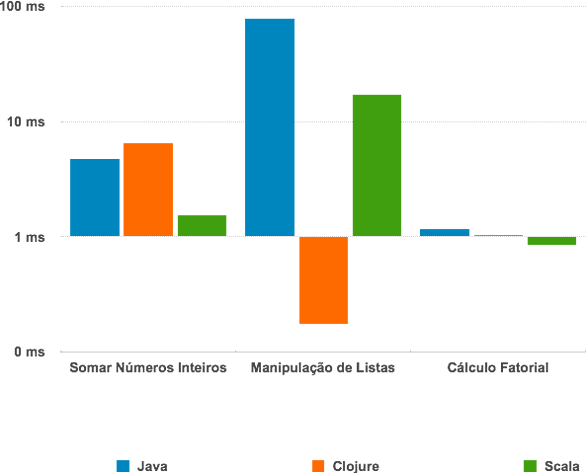
\includegraphics[width=1\textwidth]{imagem/graficos/grafico-programas.png}
      % Caption centralizada
      \captionsetup[grafico]{justification=centering}
      % Fonte
      \captionfont{\small{\textbf{\\Fonte: Dados da pesquisa}}}
    \end{grafico}

  \subsection{Linhas de Código}

    Para analisar a legibilidade de cada programa foi utilizado a quantidade de linhas de código como uma medida. As linhas que não continham nenhum caractere não foram acrescentadas a tabela a seguir.

    \begin{table}[htb] % [htb]-> here, top, bottom
       \centering   % tabela centralizada
       \large       % tamanho da fonte
       \setlength{\arrayrulewidth}{2\arrayrulewidth}  % espessura da  linha
       \setlength{\belowcaptionskip}{10pt}  % espaço entre caption e tabela
       \caption{\it Linhas de Código Utilizada Por Cada Programa}
       \begin{tabular}{|l|r|r|r|} % c=center, l=left, r=right
          \hline
          Programa & Java & Clojure & Scala \\
          \hline \hline
          Somar Números Inteiros & 12 & 10 & 9 \\
          \hline
          Manipulação de Listas & 16 & 10 & 8 \\
          \hline
          Cálculo Fatorial & 16 & 13 & 10 \\
          \hline
       \end{tabular}
    \end{table}

    Os melhores (menores) tempos de cada programa em cada linguagem de programação foram utilizados para compor o gráfico a seguir.

    \begin{grafico}[H]
      % Alterar espaçamentos antes e depois do caption
      \setlength{\abovecaptionskip}{5pt}
      \setlength{\belowcaptionskip}{0pt}
      % Caption
      \caption[Linhas de código por cada linguagem de programação]
        {Linhas de código por cada linguagem de programação}
      \centering
      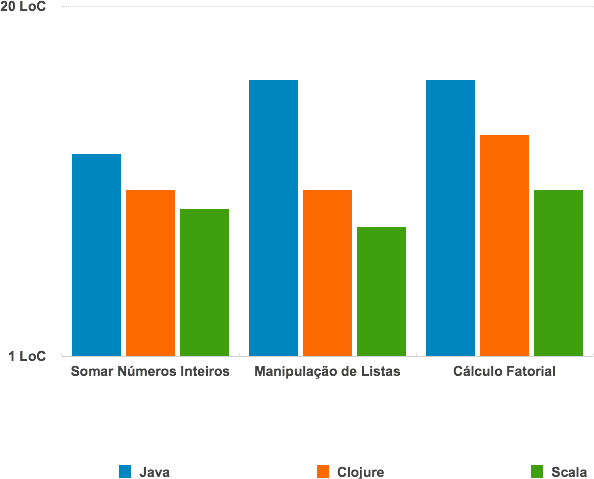
\includegraphics[width=1\textwidth]{imagem/graficos/grafico2-programas.png}
      % Caption centralizada
      \captionsetup[grafico]{justification=centering}
      % Fonte
      \captionfont{\small{\textbf{\\Fonte: Dados da pesquisa}}}
    \end{grafico}

\chapter{Conclusão}

\vspace{-1.9cm}

  A linguagem de programação Java é uma linguagem muito popular e muito utilizada para se construir programas das mais diversas finalidades. Com o passar do tempo, mesmo com a evolução tanto da linguagem Java como da máquina virtual Java, é possível notar que em determinados tipos de algoritmos a linguagem Java atrapalha ou impede o desenvolvedor de escrever programas de forma mais concisa e mantendo um bom desempenho, principalmente em códigos executados de forma concorrente ou que precisam iterar sobre coleções de objetos realizando agrupamentos ou filtros.

  Para desenvolvedores com bom conhecimento sobre a linguagem de programação Java e que não possuem conhecimento sobre nenhum dialeto Lisp, aprender e entender um programa escrito em Scala torna-se mais fácil e intuitivo, pois embora Scala faça um forte uso do paradigma funcional, ela ainda utiliza alguns conceitos do paradigma de orientação a objetos. Um outro ponto importante é que Scala também é estaticamente tipada assim como a linguagem Java, além de que quando compara com a linguagem Clojure, Scala ainda possui uma sintaxe mais próxima da linguagem Java.

  Ao contrário da linguagem Java, as linguagens Clojure e Scala são pouco conhecidas e ainda pouco utilizadas, embora seu uso vem sendo encorajado devido a grandes empresas como Twitter, LinkedIn, Facebook e Netflix anunciarem que vem utilizando essas linguagens com grande êxito em seus sistemas.

  Em face de tudo o que foi exposto anteriormente, conclui-se que é possível obter mais desempenho com programas mais concisos fazendo uso de linguagens que utilizam o paradigma de programação funcional dentro da máquina virtual Java, assim como foi visto nos capítulos introdutórios sobre o paradigma funcional e sobre as linguagens Clojure e Scala.


%%%%%%%%%%%%%%%%%%%%%%%%%%%% PÓS-TEXTUAIS %%%%%%%%%%%%%%%%%%%%%%%%%%
% Bibliografia no arquivo 'Monografia.bib'
% Alterar o título das referências para somente 'Referências'
\renewcommand{\bibname}{Referências}
\bibliographystyle{abnt-alf}
\bibliography{Monografia}

% Para forçar que os apêndices e anexos comecem no anverso
%\setboolean{@openright}{true}

% \apendice
% \begin{apendice}
% \include{pos-texto/apendiceA}
% \end{apendice}

% \anexo
% \include{pos-texto/anexo}

\end{document}
